\usepackage[italian]{babel}
\usepackage[utf8]{inputenc}
\usepackage{kmath,kerkis}
\usepackage[T1]{fontenc}
\usepackage{color}
\usepackage{hyperref}
\usepackage[absolute, overlay]{textpos}

% fonts
\usefonttheme{serif}
\usefonttheme{structurebold}

% style
\usebackgroundtemplate{
\includegraphics[width=\paperwidth]{images/background}}
\setbeamertemplate{navigation symbols}{}
\definecolor{purple}{RGB}{147,10,0}
\setbeamercolor{structure}{fg=purple}
\setbeamertemplate{items}[circle]
\setbeamercolor*{item}{fg=black}

\newcommand{\highlight}[1]{{\color{purple} \emph{#1}}}

\title{ Extreme \\ Project Evaluation }

\author{
	Jacopo Franzoi \\
	{\scriptsize jacopo.franzoi@gmail.com } \\
	{\scriptsize \href{http://jacopo.franzoi.googlepages.com/}{http://jacopo.franzoi.googlepages.com} \\ }
}

\date{
	Italian Agile Day \\
	Milano, 24 Novembre 2012
}

\begin{document}
	
	\begin{frame}
		\titlepage
		
		\note{ benvenuti, chi sono, cosa ho fatto, di cosa parlo }
	\end{frame}	

	\begin{frame}{Valutazione di Progetti}
		\begin{quote}
			{\small "<{How can you plan a project if you only have a week? [..] You don't have enough time to write a complete set of stories [..] You don't have time to write prototypes so you can estimate the stories from experience}">}
		\end{quote}
		\hfill {\scriptsize K.Beck, Extreme Programming Explained - 1st Edition}

		\begin{itemize}
			\item Scenari
			\begin{itemize}
				\item Budgeting, pre-sales
				\item Studio di fattibilità
				\item Offerta commerciale
			\end{itemize}
		\end{itemize}
		
		\note[item]{ ci viene chiesto di valutare la realizzazione di un progetto software. non abbiamo molto tempo per rispondere, non vogliamo investire troppo tempo per rispondere, ma la risposta deve essere un'indicazione attendibile. }
		\note[item]{ indicazione di budget per potenziale cliente o cliente esistente, indicazione dei tempi di realizzazione per progetti interni }
	\end{frame}


	\begin{frame}{Cosa propone XP?}
		\begin{itemize}
			\item Planning in Extreme Programming
			\begin{itemize}
				\item \highlight{Strategia}: esplorazione, commitment, steering
				\item \highlight{Valori}: feedback, semplicità, comunicazione
			\end{itemize}
		\end{itemize}

		\begin{itemize}
			\item E per la \highlight{valutazione} di progetti?
			\begin{itemize}
				\item Granularità grossa (scope, stime)
				\item Esperienza pregressa
				\item Report conciso ($1/2$ - 2 giorni)
				\item Planing Game al kick-off
			\end{itemize}
		\end{itemize}
		
		\begin{center}
			\textbf{Esplorazione, Commitment, Reporting}
		\end{center}
	\end{frame}


	\begin{frame}{Esplorazione: Brainstorming}
		\begin{columns}[T]
		    \begin{column}{.5\textwidth}
				\begin{itemize}
					\item Guida il cliente
					\item Materiale esitente
					\begin{itemize}
						\item Presentazioni
						\item Documentazione
						\item Siti web
					\end{itemize}
				\end{itemize}	

				\begin{itemize}
					\item \textbf{Mappa mentale}
				\end{itemize}
		    \end{column}
		    \begin{column}{.5\textwidth}
				\hspace*{-0.4cm} 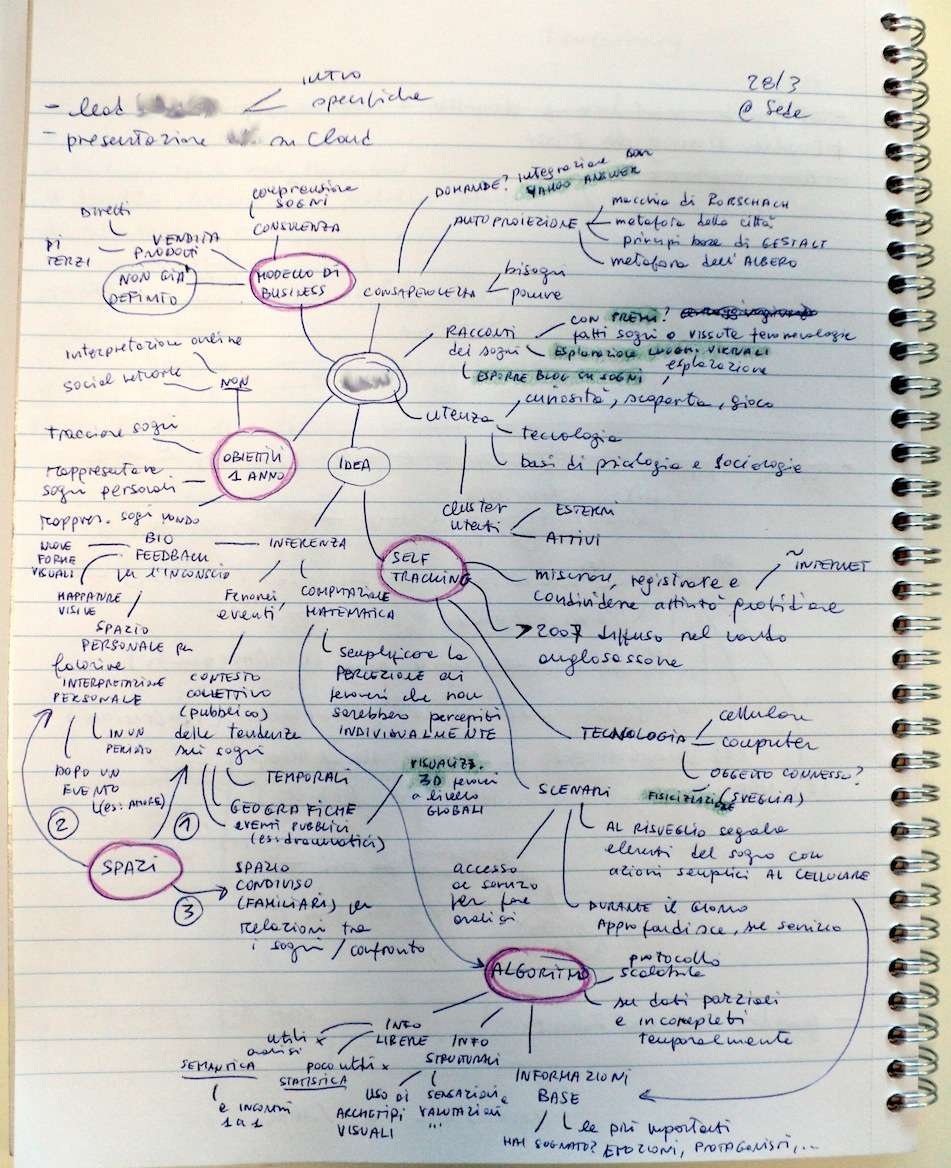
\includegraphics[scale=0.17]{images/mindmap-1}
		    \end{column}
		 \end{columns}
	\end{frame}
	
	\begin{frame}{Esplorazione: Mappa Mentale}
		\begin{columns}[T]
		    \begin{column}{.5\textwidth}
				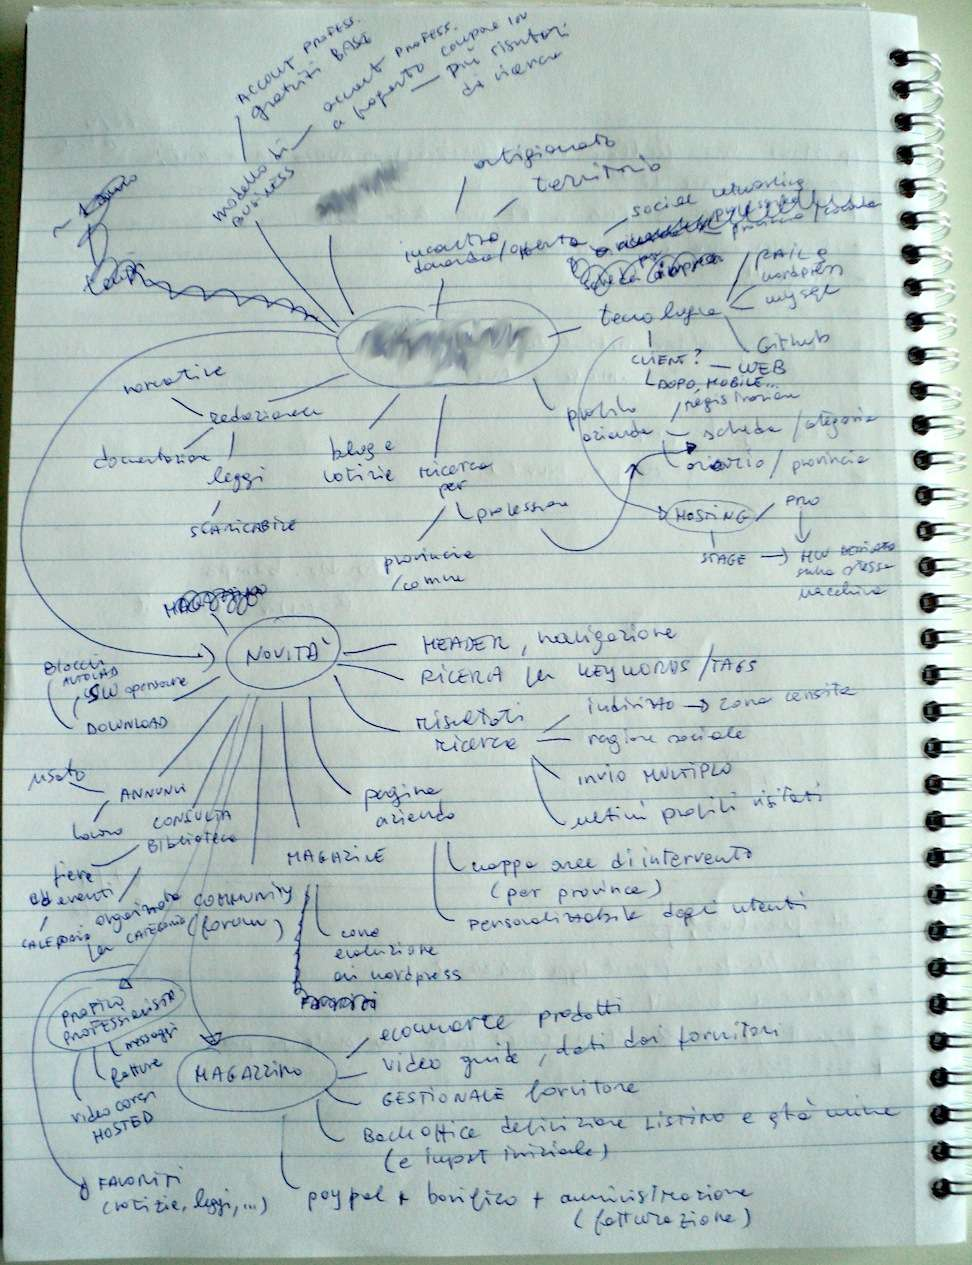
\includegraphics[scale=0.16]{images/mindmap-3}
		    \end{column}
		    \begin{column}{.5\textwidth}
				\hspace*{-0.4cm} 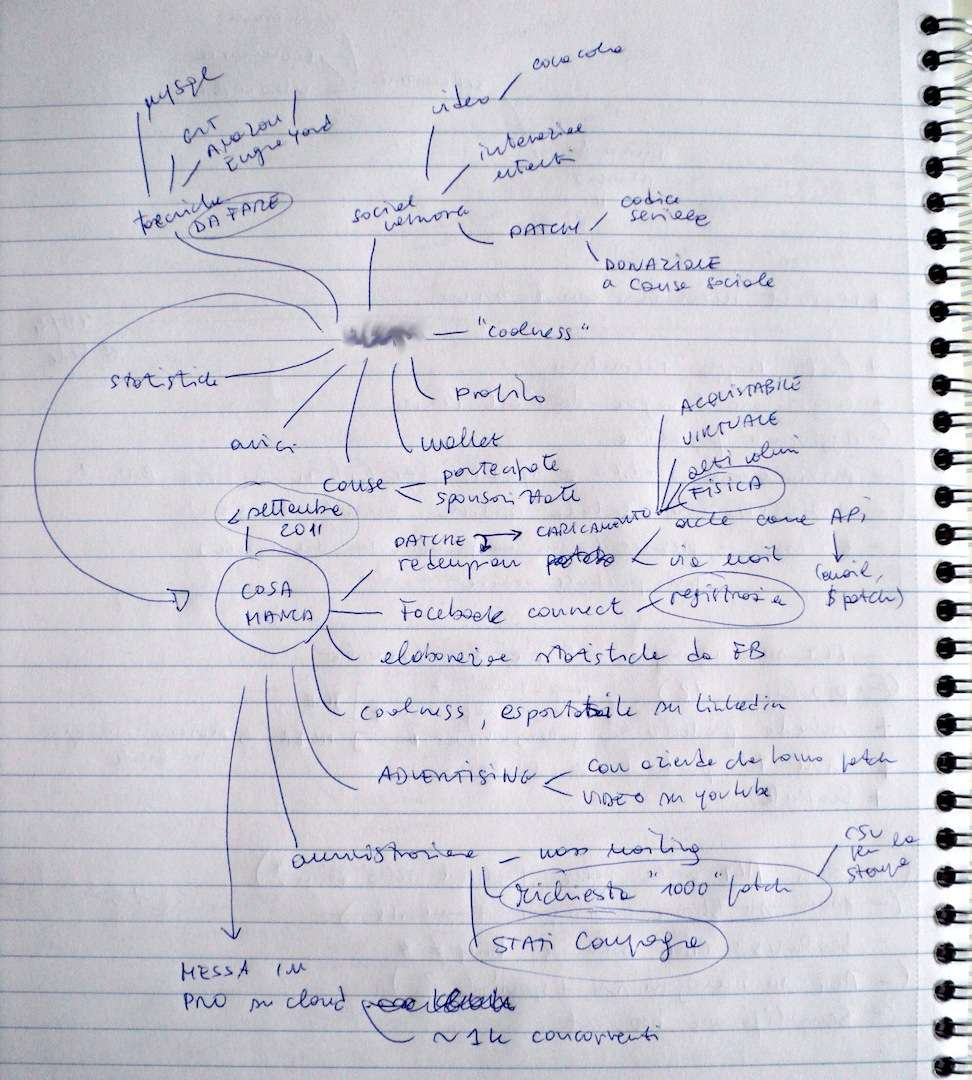
\includegraphics[scale=0.17]{images/mindmap-2}
		    \end{column}
		 \end{columns}
	\end{frame}

	\begin{frame}{Esplorazione: Cosa?}

		\begin{columns}[T]
		    \begin{column}{0.6\textwidth}

				\begin{itemize}
					\item Storie, temi
					\item Scadenze, eventi
				\end{itemize}

				\begin{itemize}
					\item \textbf{Piano di rilascio}
					\begin{itemize}
						\item Note, domande
						\item Nessuna stima
					\end{itemize}
					\item \textbf{Modello del dominio}
					\begin{itemize}
						\item Entità, relazioni
						\item Cardinalità
					\end{itemize}
				\end{itemize}
				
	    \end{column}
	    \begin{column}{0.4\textwidth}
			\hspace*{-0.9cm} 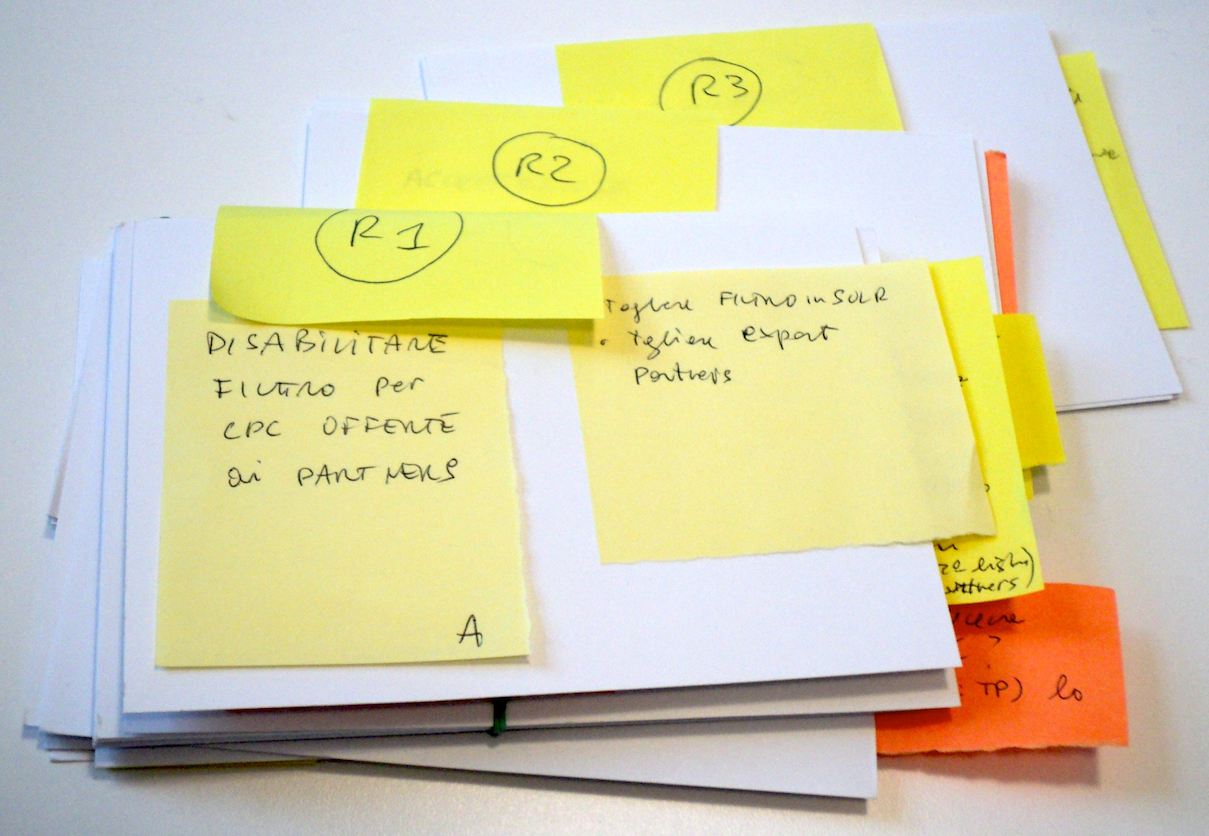
\includegraphics[scale=0.115]{images/stories}
			\\ \vspace*{0.4cm}
			\hspace*{-0.9cm} 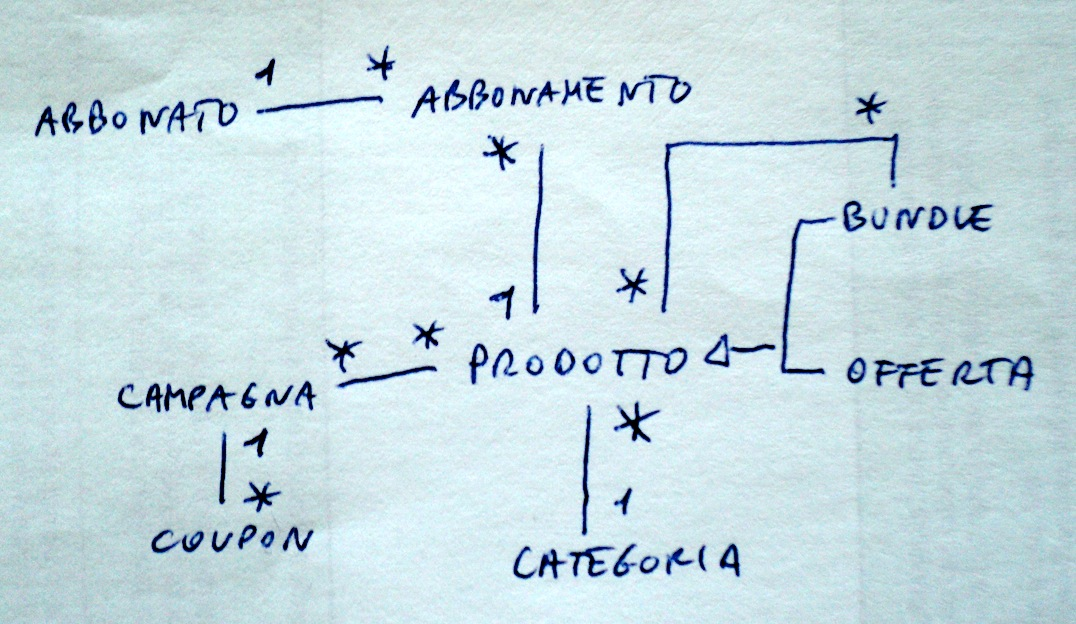
\includegraphics[scale=0.13]{images/domain-1}
	    \end{column}
	 \end{columns}
	\end{frame}
	
	\begin{frame}{Esplorazione: Modello del Dominio}
		\begin{columns}[T]
		    \begin{column}{.5\textwidth}
				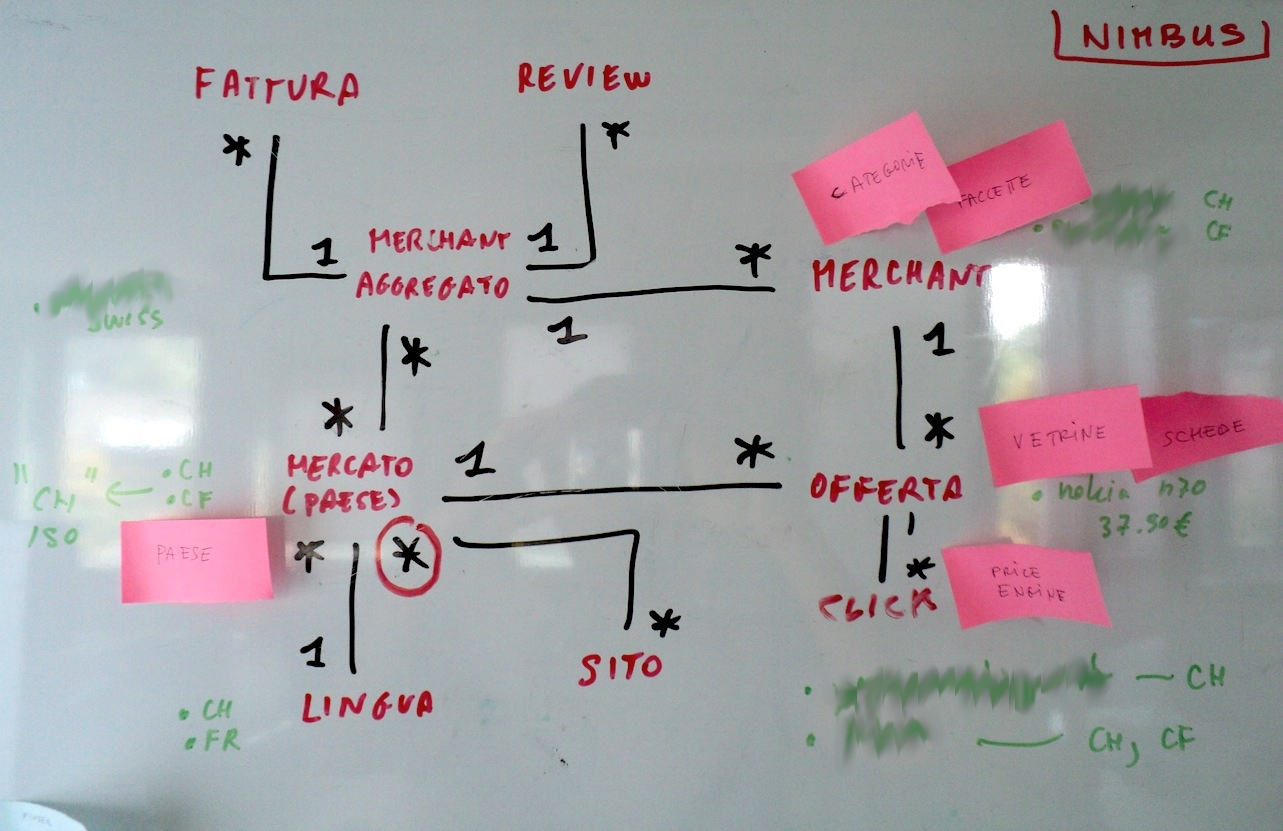
\includegraphics[scale=0.12]{images/domain-2}
				\\ \vspace*{0.4cm}
				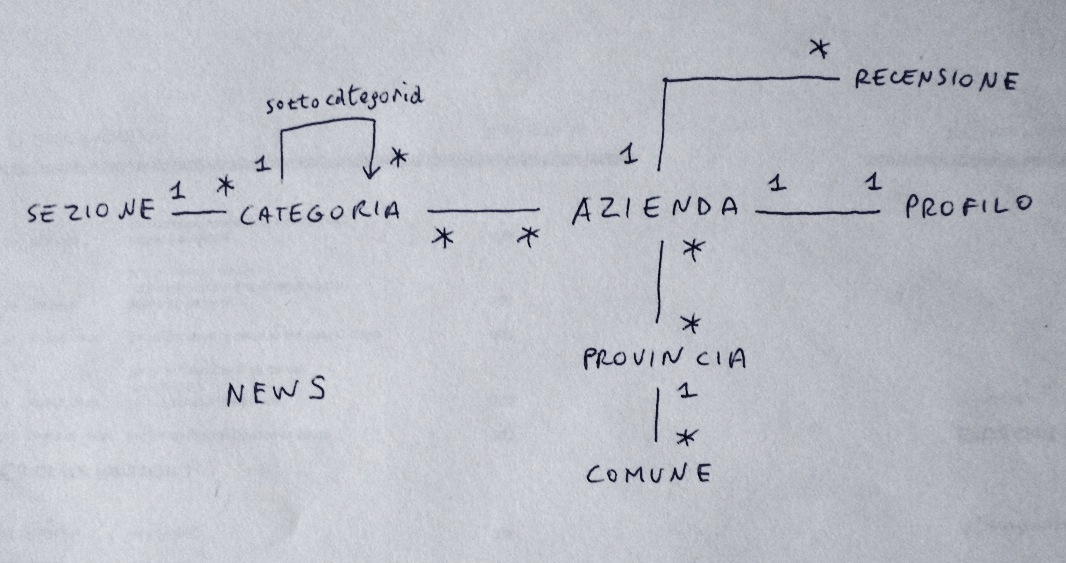
\includegraphics[scale=0.15]{images/domain-4}
		    \end{column}
		    \begin{column}{.5\textwidth}
				\vspace*{0.3cm}
				\hspace*{-0.3cm} 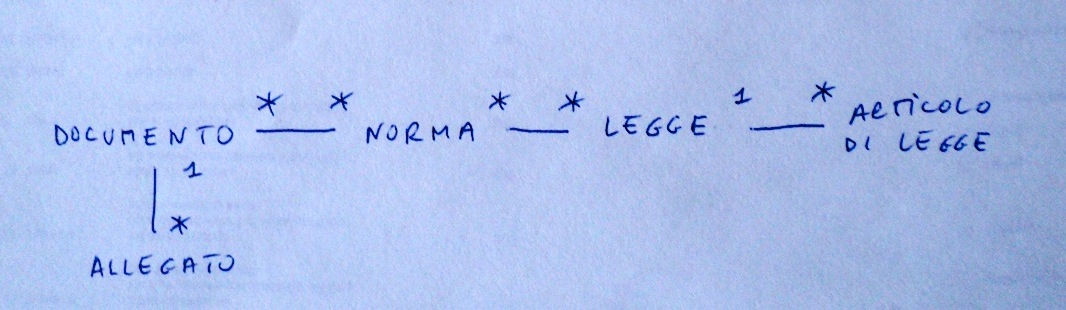
\includegraphics[scale=0.15]{images/domain-5}
				\\ \vspace*{0.3cm}
				\hspace*{-0.3cm} 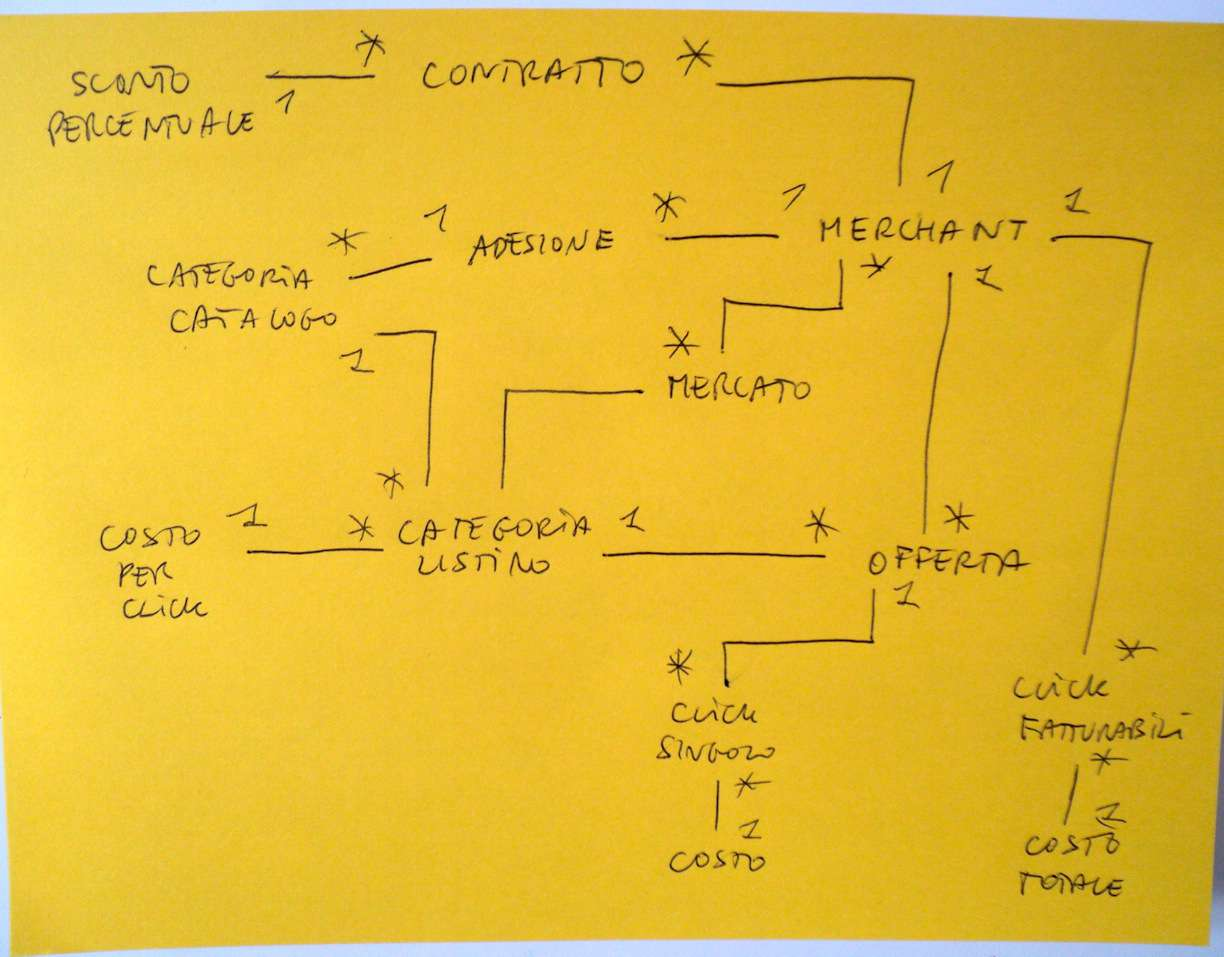
\includegraphics[scale=0.13]{images/domain-3}
		    \end{column}
		 \end{columns}
	\end{frame}

	\begin{frame}{Esplorazione: Come?}
		
		\begin{columns}[T]
		    \begin{column}{.5\textwidth}

		\begin{itemize}
			\item \textbf{Architettura Logica}
			\begin{itemize}
				\item Sistemi
				\item Interconnessioni
				\item Clients (e utenti)
			\end{itemize}
			\item \textbf{Hosting}
			\begin{itemize}
				\item In-house, cloud
				\item Pro, staging
			\end{itemize}
			\item \textbf{Spikes}
		\end{itemize}
		
	    \end{column}
	    \begin{column}{.5\textwidth}
			\hspace*{-0.6cm} 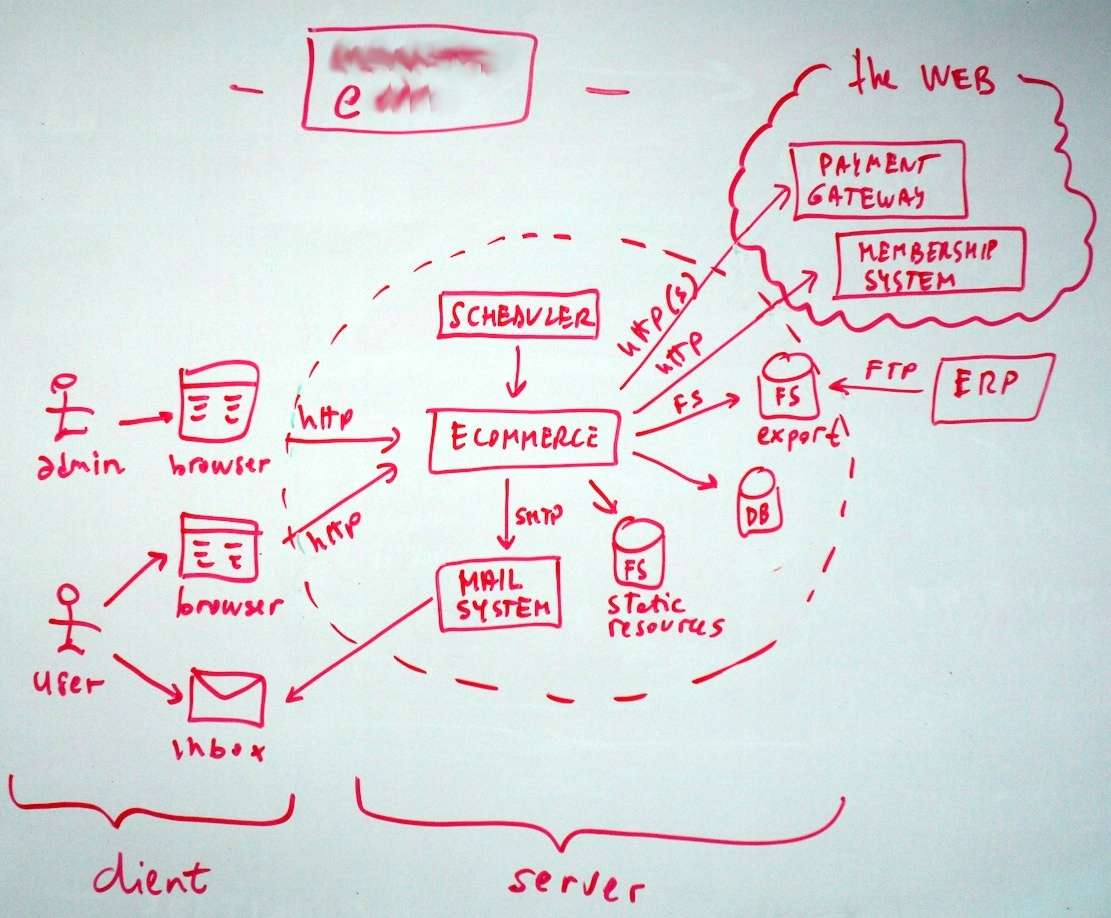
\includegraphics[scale=0.15]{images/architecture-1}
	    \end{column}
	 \end{columns}

	\end{frame}
	
	\begin{frame}{Esplorazione: Architettura Logica}
		\begin{columns}[T]
		    \begin{column}{.5\textwidth}
				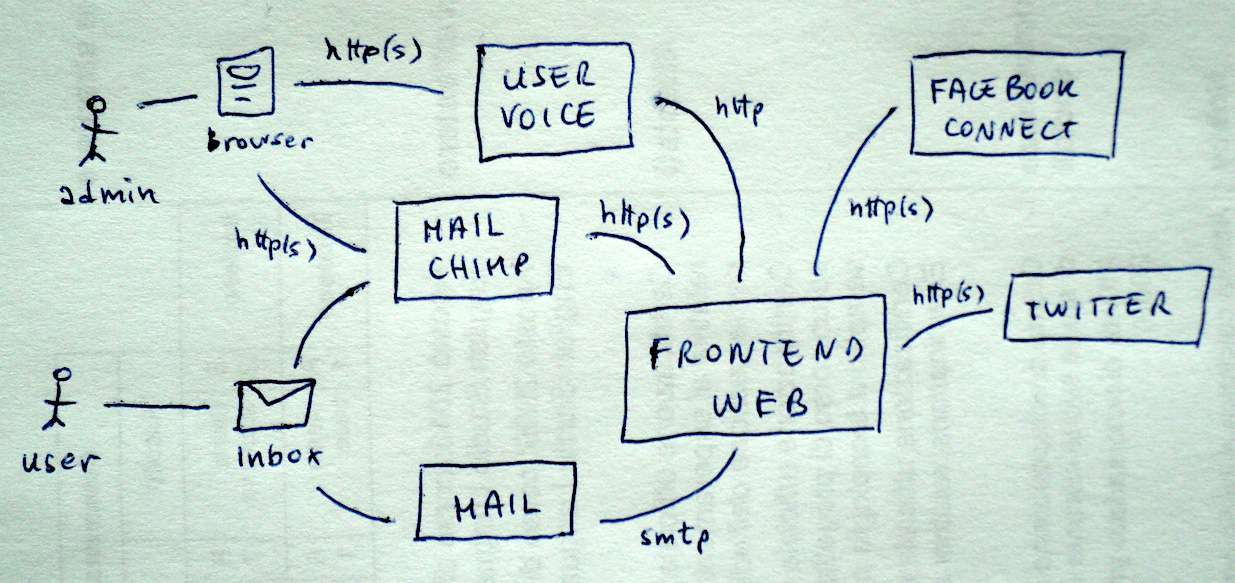
\includegraphics[scale=0.13]{images/architecture-2}
				\\ \vspace*{0.2cm}
				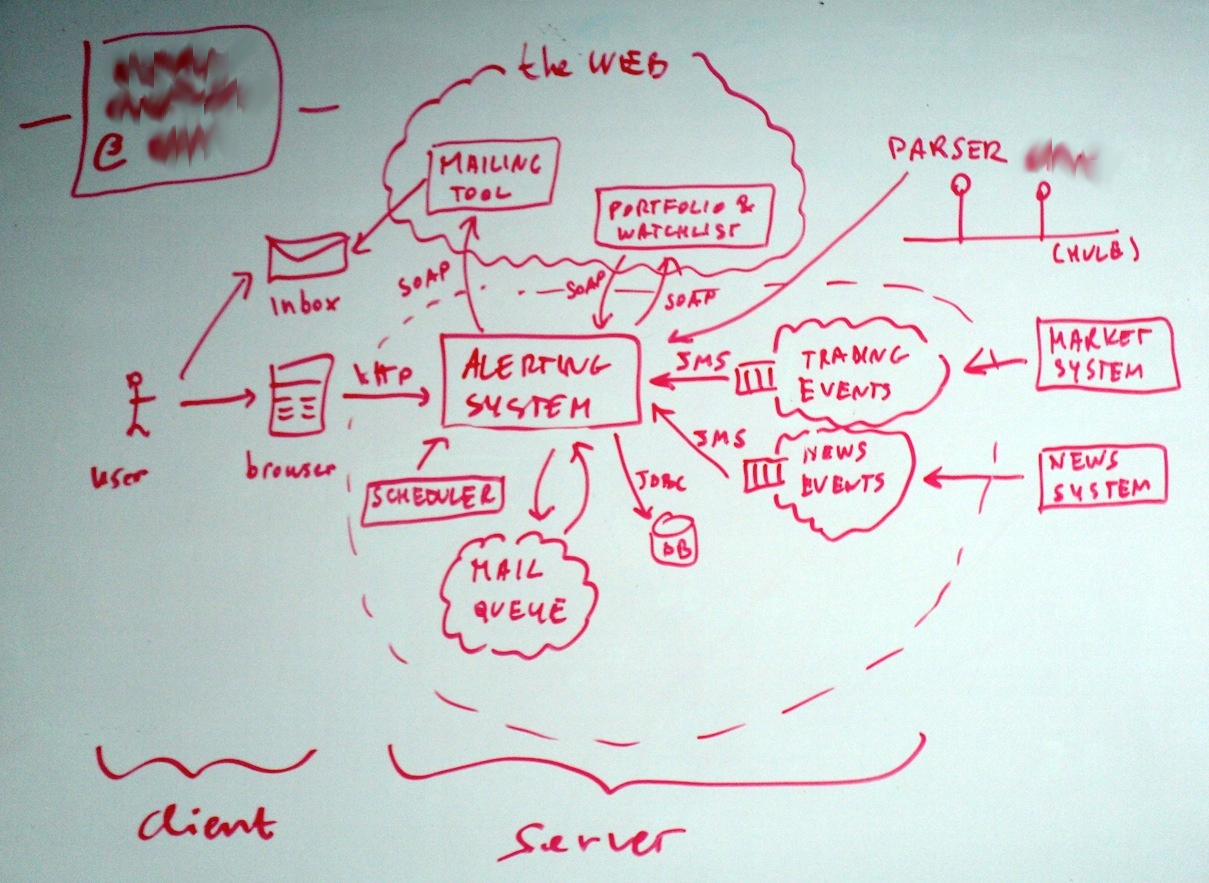
\includegraphics[scale=0.135]{images/architecture-3}
		    \end{column}
		    \begin{column}{.5\textwidth}
				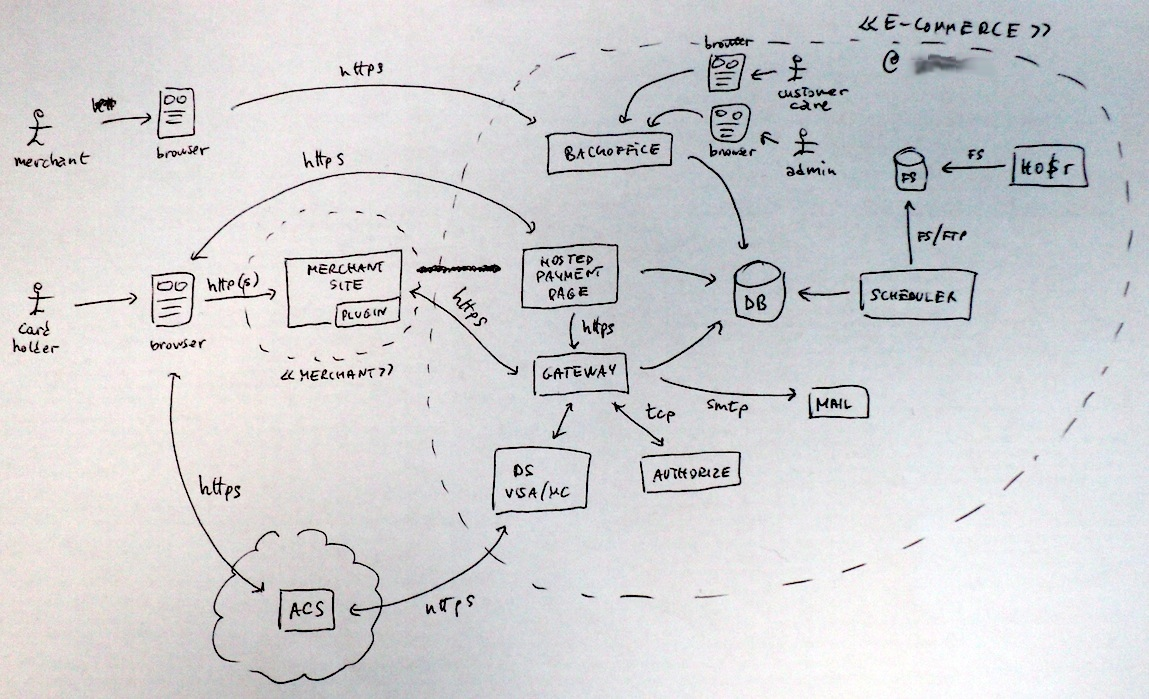
\includegraphics[scale=0.13]{images/architecture-5}
				\\ \vspace*{0.2cm}
				\hspace*{0.2cm} 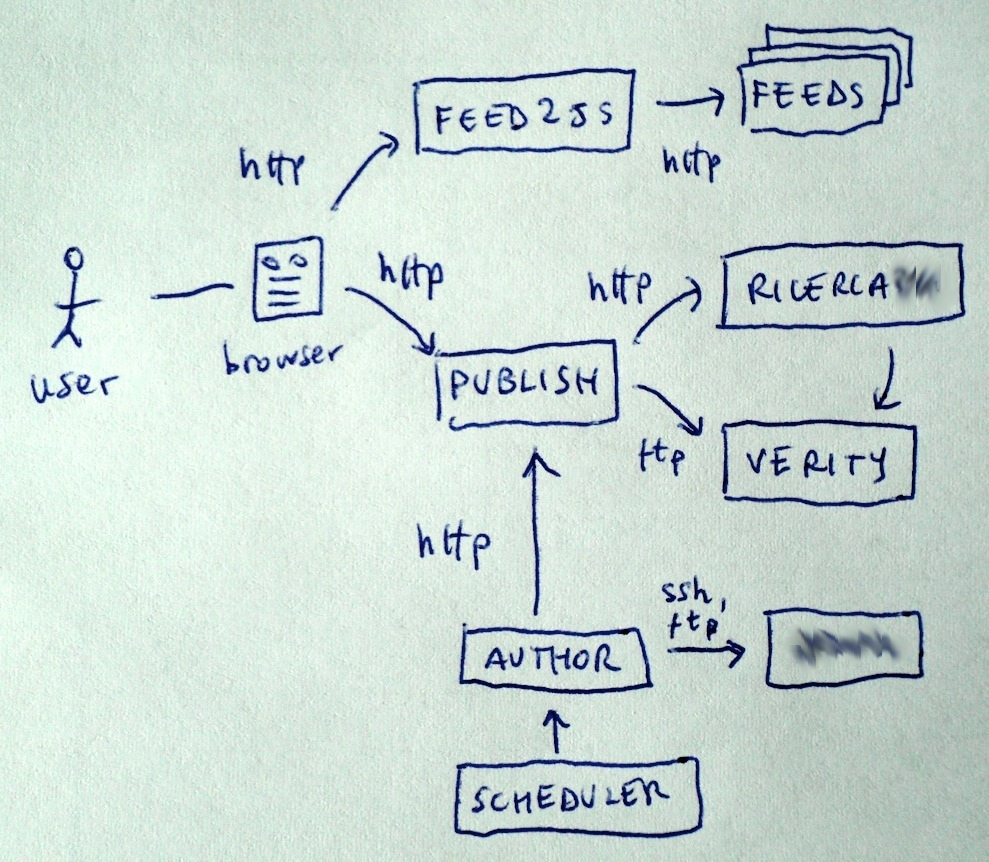
\includegraphics[scale=0.13]{images/architecture-4}
		    \end{column}
		 \end{columns}
	\end{frame}

	\begin{frame}{Commitment: Stima}
		
		\begin{columns}[T]
		    \begin{column}{.5\textwidth}
		
				\begin{itemize}
					\item Complessità
					\begin{itemize}
						\item Mimina, 50\%
						\item Massima, 90\%
					\end{itemize}
					\item Incertezza
					\begin{itemize}
						\item Buffer ($ \sigma $)
					\end{itemize}
				\end{itemize}

				\begin{itemize}
					\item \textbf{Effort}
					\begin{itemize}
						\item Minima + Buffer
					\end{itemize}
				\end{itemize}
		
		    \end{column}
		    \begin{column}{.5\textwidth}
				\hspace*{-0.8cm} 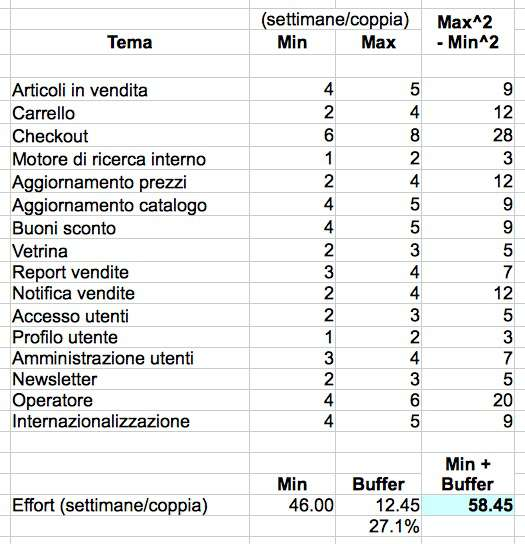
\includegraphics[scale=0.28]{images/effort}
				\\ \vspace*{0.2cm}
				{\small $ \sigma = \sqrt[2] { \sum \left ( max^{2} - min^{2} \right ) } $}
		    \end{column}
		 \end{columns}
	
	\end{frame}

	\begin{frame}{Commitment: Piano di Rilascio}

		\begin{columns}[T]
		    \begin{column}{.5\textwidth}

				\begin{itemize}
					\item Composizione team
					\begin{itemize}
						\item Coppie, coach
						\item Velocità prevista
					\end{itemize}
				\end{itemize}

				\begin{itemize}
					\item \textbf{Elapsed}
					\begin{itemize}
						\item Originale
						\item Per il business
					\end{itemize}
				\end{itemize}
		
	    	\end{column}
		    \begin{column}{.5\textwidth}
				\hspace*{-0.1cm} 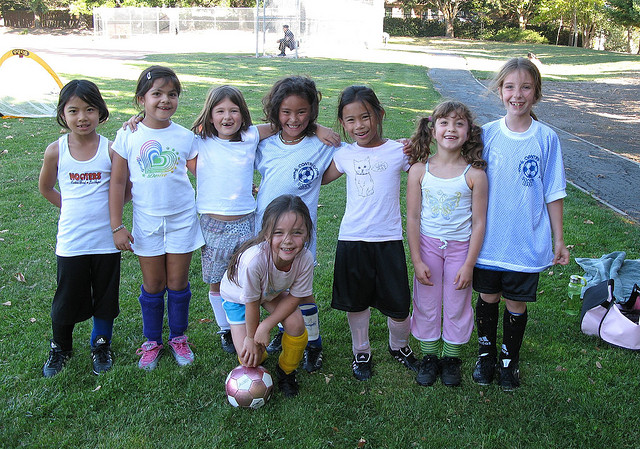
\includegraphics[scale=0.55]{images/team}
				\\ \vspace*{0.2cm}
				\hspace*{-0.2cm} 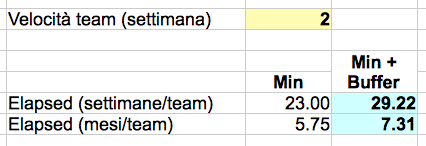
\includegraphics[scale=0.35]{images/elapsed}
		    \end{column}
		\end{columns}

		\vspace*{1cm}
		{\footnotesize \highlight{\href{http://www.flickr.com/photos/kimberlyjennery/1210060984/}{http://www.flickr.com/photos/kimberlyjennery/1210060984/}}}

	\end{frame}
	
	\begin{frame}{Commitment: Costi}
		
		\begin{columns}[T]
		    \begin{column}{.5\textwidth}
			
				\begin{itemize}
					\item Sviluppo
					\item Hosting
						\begin{itemize}
							\item Previsione
						\end{itemize}
					\item Servizi
					\begin{itemize}
						\item Monitoring
						\item Mailing
					\end{itemize}
				\end{itemize}
				
				\vspace*{0.2cm}
				\hspace*{0.5cm} 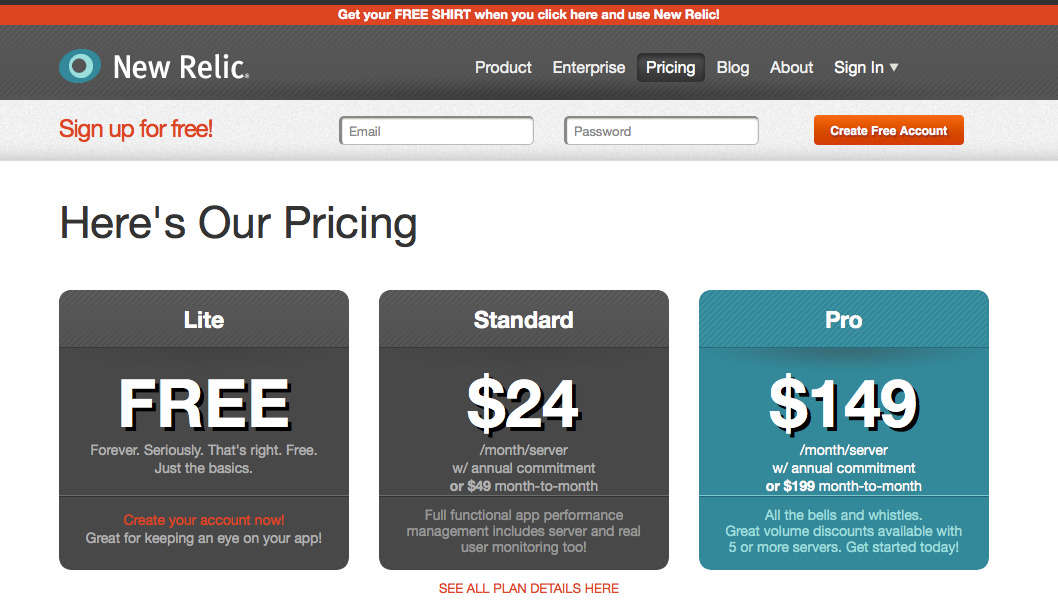
\includegraphics[scale=0.14]{images/costs-3}
    		\end{column}

	    \begin{column}{.5\textwidth}
			\hspace*{-0.8cm} 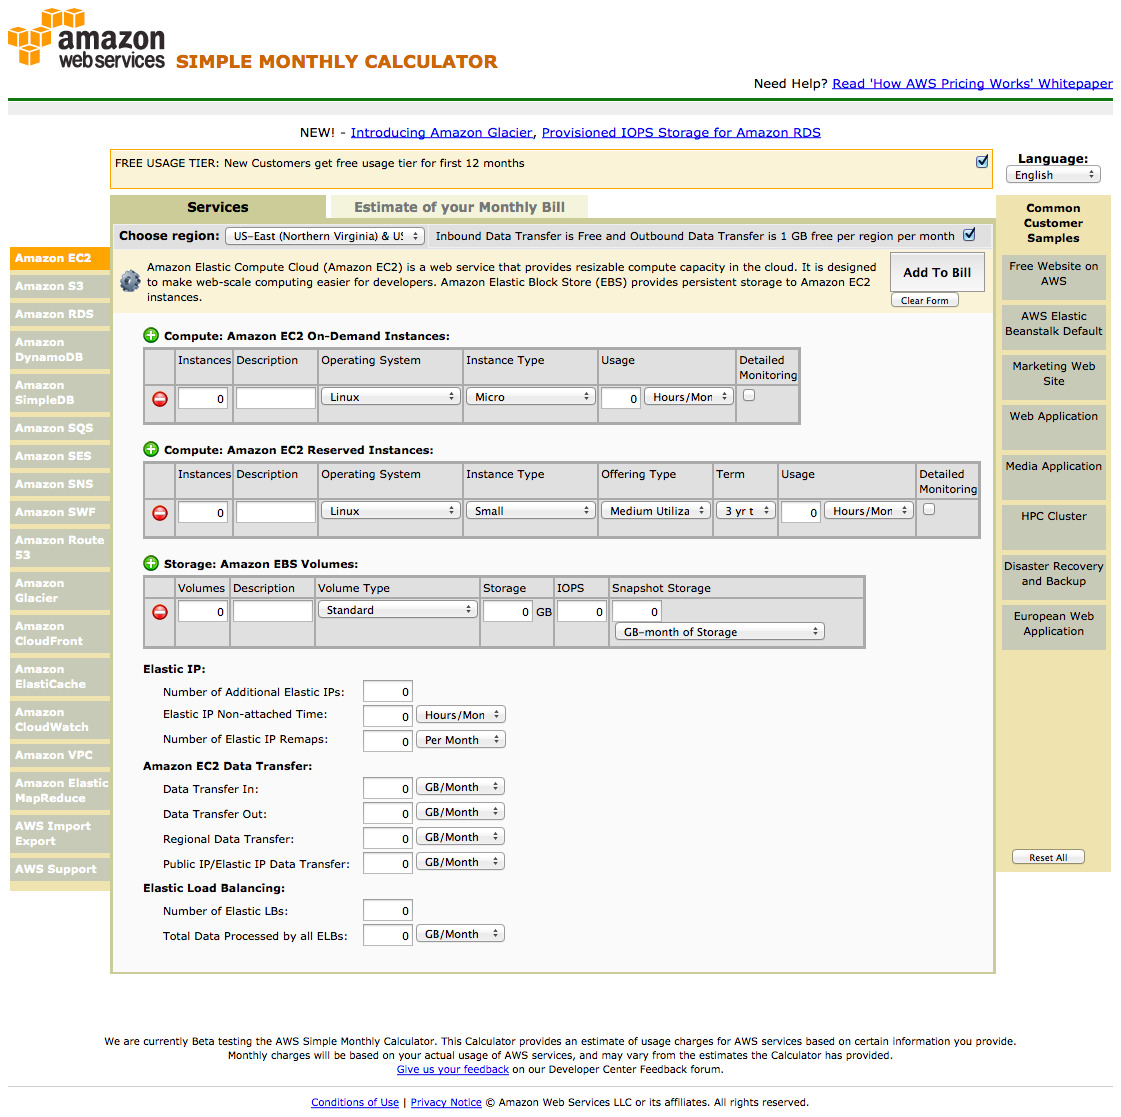
\includegraphics[scale=0.13]{images/costs-1}
			\\ \vspace*{-1cm}
			\hspace*{0.2cm} 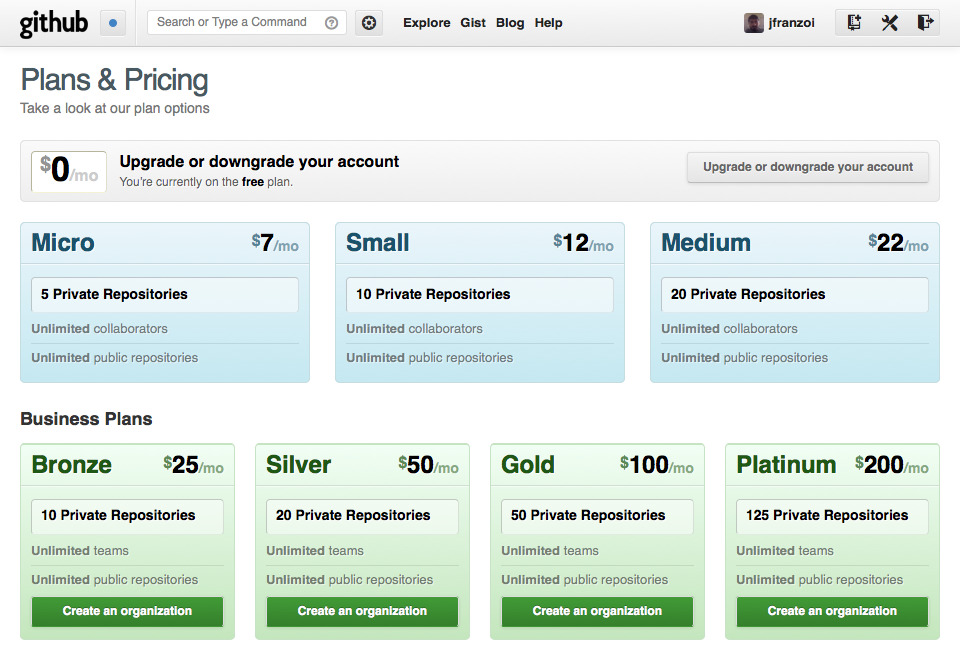
\includegraphics[scale=0.15]{images/costs-2}			
		    \end{column}
		\end{columns}

	\end{frame}
	
	\begin{frame}{Reporting: Non un \emph{contratto}!}
		\begin{itemize}
			\item \textbf{Introduzione}
			\begin{itemize}
				\item Il team, il cliente
				\item Date incontri
			\end{itemize}

			\item \textbf{Valutazione}
			\begin{itemize}
				\item Narrativa, modello del dominio
				\item Piano di rilascio
				\item Tabelle riassuntive: effort, elapsed
			\end{itemize}

			\item \textbf{Soluzione tecnica}
			\begin{itemize}
				\item Architettura logica, hosting
			\end{itemize}

			\item \textbf{Costi}
			\begin{itemize}
				\item Tabella riassuntiva
			\end{itemize}
		\end{itemize}
	\end{frame}
	
	\begin{frame}{Sì, ma...}
		\begin{itemize}
			\item \highlight{Per prodotti e progetti interni?}
				\begin{itemize}
					\item Costi e hosting impliciti
					\item Focus su effort ed elapsed
				\end{itemize}
			\item \highlight{Chi paga per questa valutazione?}
				\begin{itemize}
					\item Preventivi (fornitore) vs. kick-start (cliente)
				\end{itemize}
			\item \highlight{Per il contratto?}
				\begin{itemize}
					\item Win-win, incrementale
				\end{itemize}
			\item \highlight{Cosa avviene al kick-off?}
				\begin{itemize}
					\item Planning Game iniziale
					\item Steering, convalidare valutazione
				\end{itemize}
		\end{itemize}
	\end{frame}

	\begin{frame}{Cosa Portare a Casa}
		\hspace*{-0.5cm} 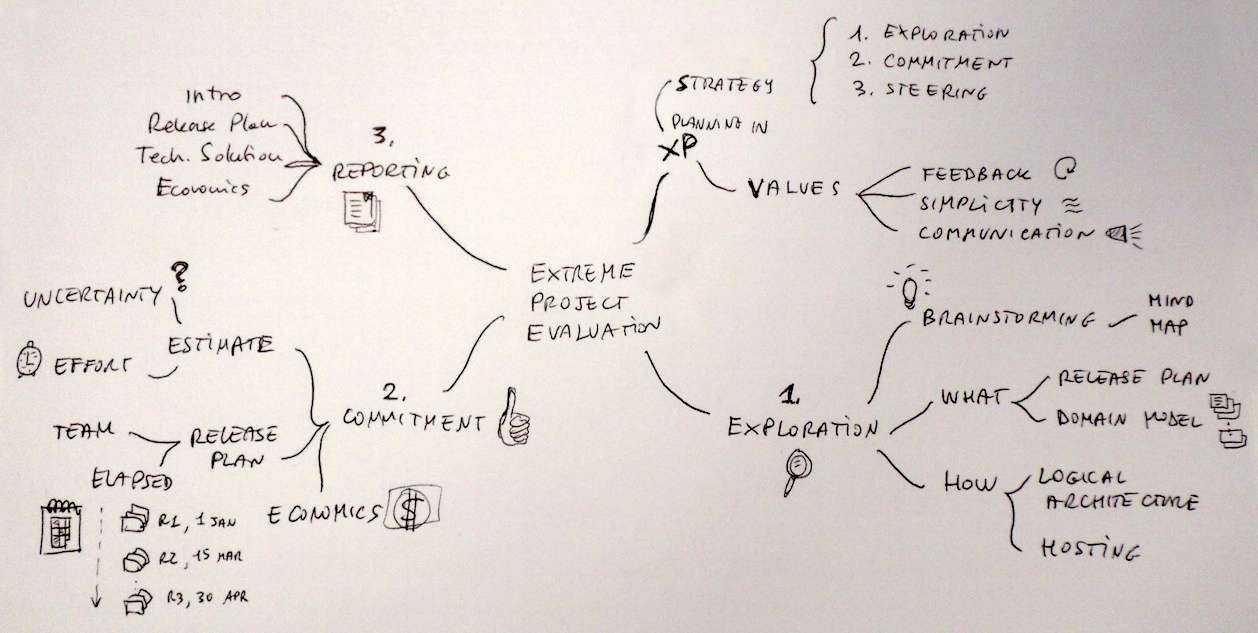
\includegraphics[scale=0.26]{images/takeaway}
	\end{frame}
	
	\begin{frame}{Per Approfondire}
		\begin{itemize}	
			\item Pianificazione e valori in XP
				\begin{itemize}
					\item {\small K.Beck \highlight{Extreme Programming Explained - 1st ed}}
				\end{itemize}

			\item Stima e incertezza
				\begin{itemize}
					\item {\small M.Cohn \highlight{Agile Estimating and Planning}}
				\end{itemize}

			\item Architettura logica
				\begin{itemize}
					\item {\small N.Pryce \highlight{\href{http://www.natpryce.com/articles/000755.html}{Test-Driven Development of Asynchronous Systems}}}
					\item {\small P.Clements et al. \highlight{Documenting Software Architectures: Views and Beyond - 2nd ed}}
				\end{itemize}

			\item Contratti
				\begin{itemize}
					\item {\small J.Franzoi \highlight{\href{http://jfranzoi.wordpress.com/2011/11/23/mas-vale-tarde-que-nunca/}{Mas vale tarde que nunca}}}
				\end{itemize}
		\end{itemize}
		
		
	\end{frame}

\end{document}